\section{P2: Gestión de Productos con Python}

\subsection{Carga con API Pública}

Primero, completamos la función de \textit{fetching} de datos.

\begin{minted}{python}
def fetch_all_categories(self, base_url):
    # cada objeto en base_url tiene:
    # slug, name, url
    response = self.fetch_json_data(base_url)
    self.db.categorias.insert_many(response)
\end{minted}

Con esta función, obtenemos todas las categorías de productos desde la API, y las
insertamos en la colección \texttt{categorias} en Mongo.

Luego, completamos la función de obtención de productos.

\begin{minted}{python}
def fetch_all_products(self):
documents = self.db.categorias.find()
for doc in documents:
    response = self.fetch_json_data(doc["url"])
    print(f"Fetched {len(response["products"])} items for category {doc["name"]}")
    self.db.productos.insert_many(response["products"])
\end{minted}

Después, probamos la conexión a nuestro Atlas cluster, reemplazando el URI por el \textit{connection string}
que nos da el app web.

\begin{figure}[H]
    \centering
    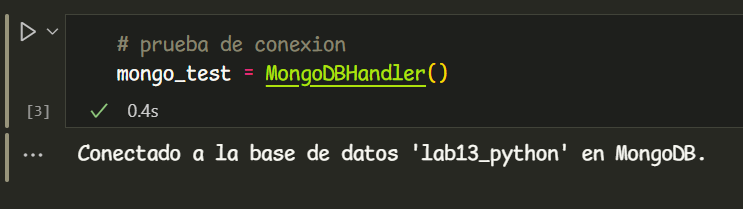
\includegraphics[width=0.6\textwidth]{./p2_pruebaconexion.png}
    \caption{Conexión a MongoDB desde Python}\label{fig:pruebaconexion}
\end{figure}

Luego, encapsulamos la funcionalidad de \textit{fetching} en una función, la cual sólo se
ejecuta una vez para cargar los datos a nuestro cluster.

\begin{figure}[H]
    \centering
    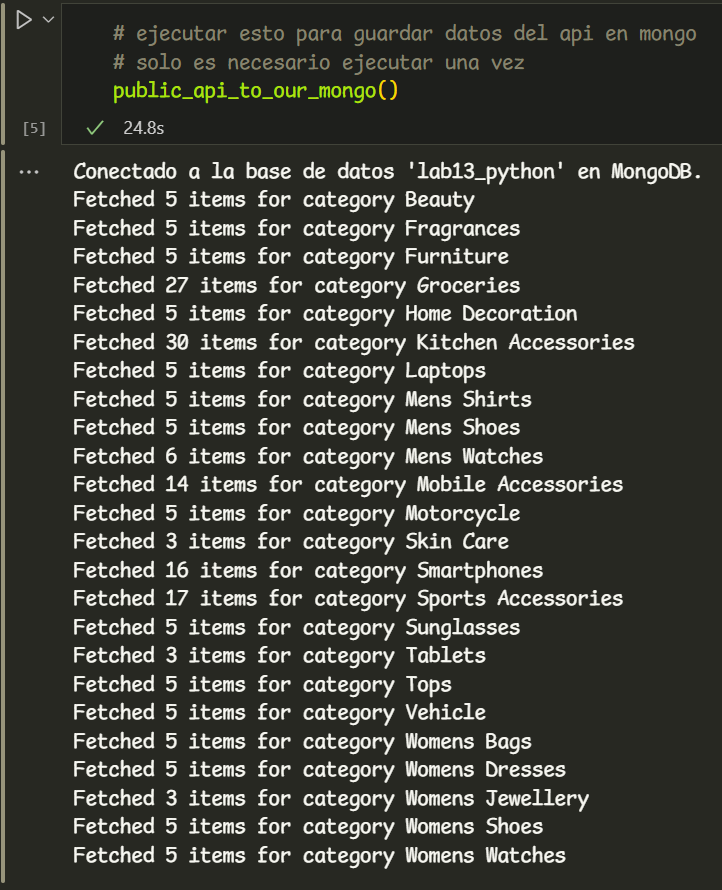
\includegraphics[width=0.6\textwidth]{./p2_fetching.png}
    \caption{Fetching de datos}\label{fig:fetching}
\end{figure}

Luego de ejecutar la función, podemos ver que los datos \hyperref[cargadatos]{se han cargado correctamente}.

\subsection{CRUD y Filtrado}

Luego de cargar los datos a Mongo, implementamos las funciones de CRUD y filtrado que se solicitaron.

\begin{figure}[H]
    \centering
    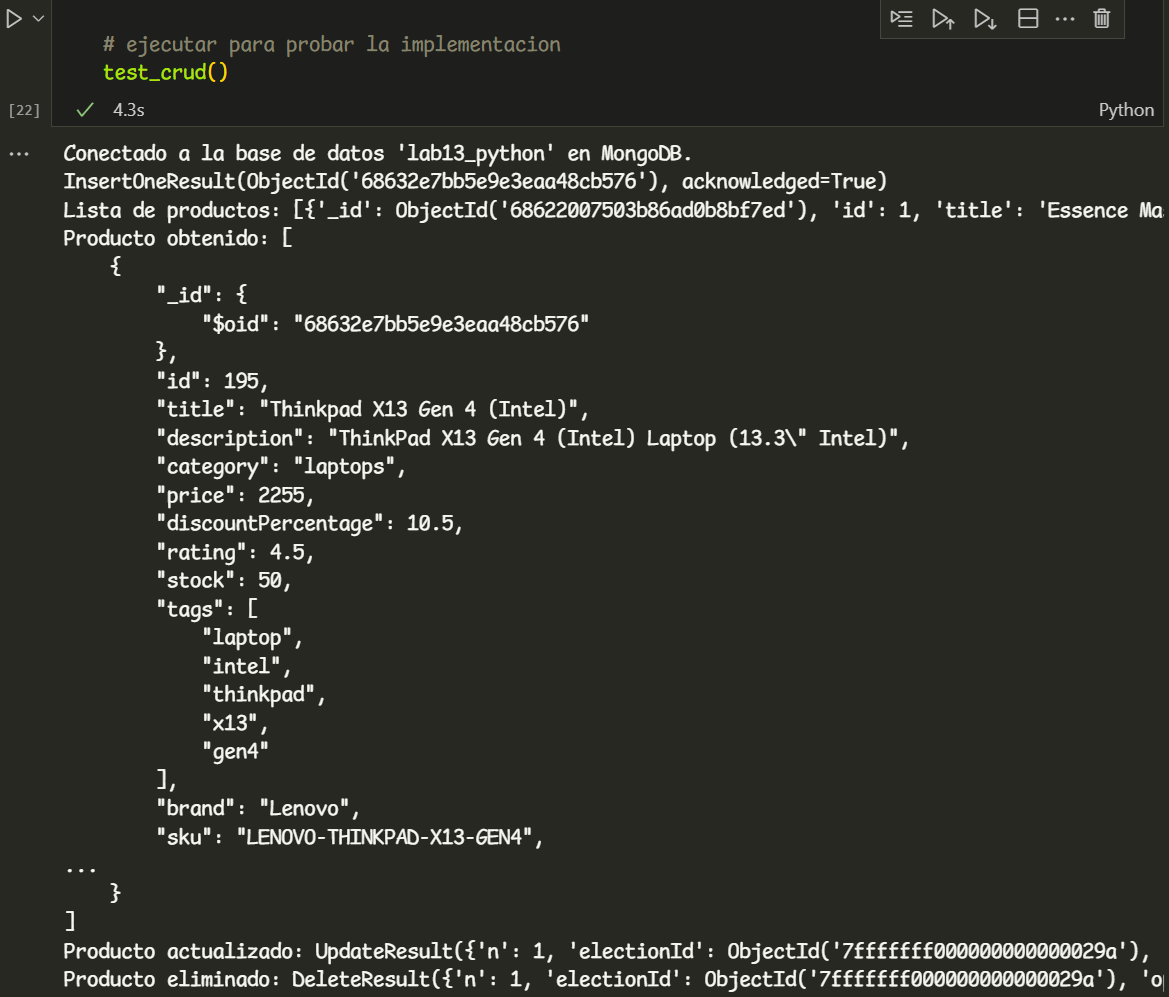
\includegraphics[width=0.6\textwidth]{./p2_crud.png}
    \caption{CRUD desde Python}\label{fig:crud}
\end{figure}

Finalmente, ejecutamos las funciones de agregación. Los resultados se muestran a continuación:

\begin{figure}[H]
    \centering
    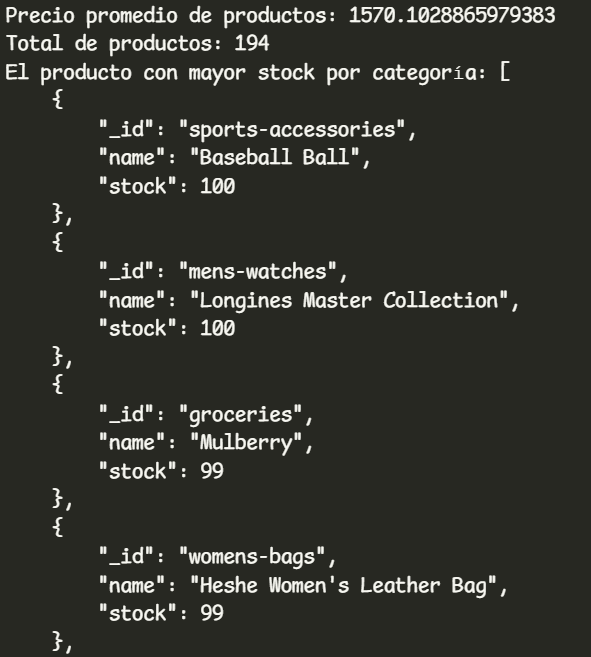
\includegraphics[width=0.4\textwidth]{./p2_agregadas.png}
    \caption{Resultado de promedio, total y máximo de productos por categoría}\label{fig:agregadas}
\end{figure}

Nota: El \textit{notebook} con la implementación de la clase \textbf{MongoDBHandler} se encuentra en el repositorio de \hyperref[repo]{GitHub} disponible
en el anexo.
